\documentclass[12pt,a4paper]{report}
\usepackage[utf8]{inputenc}
\usepackage[spanish]{babel}
\usepackage{amsmath}
\usepackage{amsfonts}
\usepackage{amssymb}
\usepackage{makeidx}
\usepackage{graphicx}
\usepackage{lmodern}
\usepackage{kpfonts}
\usepackage{fourier}
\usepackage[left=2cm,right=2cm,top=2cm,bottom=2cm]{geometry}
\begin{document}

\includegraphics[scale=0.5]{imagenes/UPZMG.jpg} 
$$\section*{Descripción de las condiciones de singularidad de manipuladores seriales}$$\\\\

Medina Rodríguez Francisco Javier\\
Ing. Mecatrónica 7°A\\
Cinemática de Robots\\\\

\section*{Conceptos}\\
Singularidad mecánica: Una posición o configuración de un mecanismo o una máquina donde el comportamiento subsecuente no se puede predecir o las fuerzas u otras magnitudes se vuelven infinitas o indeterminadas.\\\\
Configuración singular: Una configuración
singular o simplemente singularidad de un manipulador se presenta cuando los grados de
libertad del sistema -o mecanismo- cambian instantáneamente -aumentan o se reducen-, lo
cual, evidentemente, es indeseable.\\\\
Una singularidad es aquella configuracion en la que el manipulador pierde algunos de sus grados de libertad (Murray
et al., 1994; Spong et al., 2006; Craig, 1989; Siciliano et al.,
2008). Esto se traduce en que el elemento terminal pierde la
capacidad de movimiento en ciertas direcciones y en que se requieren velocidades articulares infinitas para generar velocidades lineales y angulares finitas del elemento terminal. (Hollerbach, 1985; Gottlieb, 1986) demuestran de forma independiente que cualquier manipulador serie de n > 2 GdL posee singularidades.\\

\section*{Descripción}\\
Para robots manipuladores redundantes, las singularidades
pueden obtenerse mediante dos enfoques diferentes:\\
1. Resolviendo la ecuación no lineal: 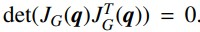
\includegraphics[scale=0.5]{imagenes/EC1.jpg} 
Esta forma es mas compleja de abordar sin usar métodos numéricos pero es la más general.\\
2. Para aquellos manipuladores redundantes con muneca esférica, las singularidades pueden desacoplarse en: singularidades de posicion, orientación y acopladas (Oetomo, 2004). Para ello se consideran las submatrices del jacobiano.\\\\

A continuacion, se resumen los principales procedimientos para obtener las direcciones singulares asociadas a las singularidades:\\

En primer lugar se procede a expresar JG(q) en los diferentes sistemas de referencia asociados a las articulaciones, esto es iJG(q) para todo i = 0, 1, . . . , 7 y se evaluan dichas matrices en cada una de las configuraciones singulares. Si aparece una fila de ceros, la direccion singular se alinea con uno de los ejes principales del sistema de
referencia {i}. Esto se debe a que la componente correspondiente de la velocidad lineal o angular del elemento terminal no podra generarse sea cual sea el vector de velocidades articulares. Si la fila de ceros es una de las
tres primeras filas, la direccion singular será la traslación
a traves del correspondiente eje del sistema de referencia {i} mientras que si la fila de ceros es una de las tres
últimas, entonces la dirección singular será la rotación alrededor del correspondiente eje de dicho sistema de referencia.\\\\
Una segunda opcion consiste en expresar JG(q) en un sistema de referencia {F} distinto de los sistemas de referencia asociados a las articulaciones. Al igual que en el
caso anterior, si en FJG(q) hay una fila de ceros, la o las
direcciones singulares estarán alineadas con algunos de los ejes de {F} ya sea impidiendo la traslación o rotación alrededor de ellos.\\\\
Se tiene el siguiente robot:\\
$$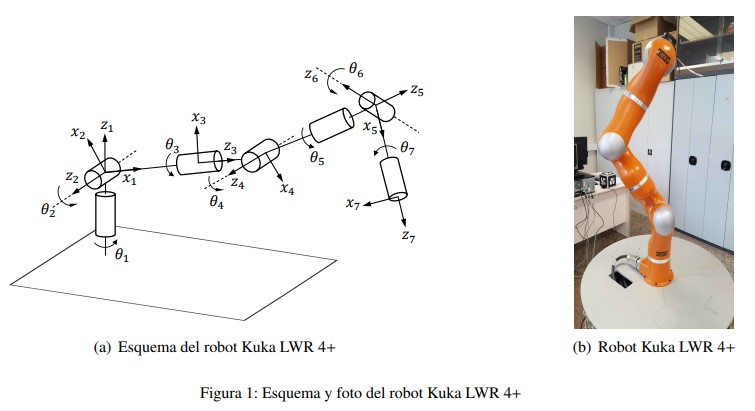
\includegraphics[scale=0.9]{imagenes/figura1.jpg}$$\\
$$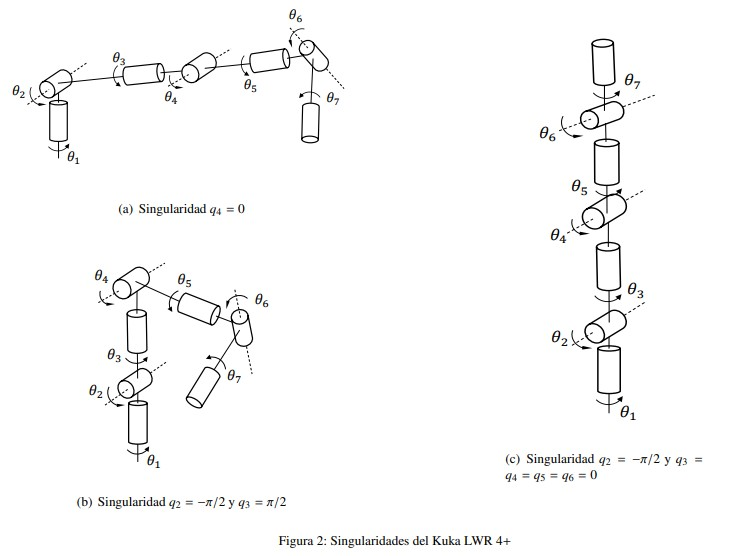
\includegraphics[scale=1]{imagenes/figura2.jpg} $$\\
\\Tomando en cuenta las figuras anteriores se pueden obtener las siguientes singularidades:\\\\

\textbf{Singularidad de posición}\\
q4 = 0\\
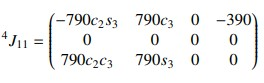
\includegraphics[scale=1]{imagenes/EC2.jpg} \\
Es claro que la direccion singular asociada es la traslacion a lo largo del eje \textit{y} del sistema de referencia 4.\\
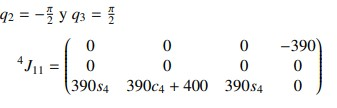
\includegraphics[scale=1]{imagenes/EC3.jpg}\\
Tambien en este caso la dirección singular asociada es la traslación a lo largo del eje \textit{y} del sistema de
referencia 4.\\\\
\textbf{Singularidad de orientación}\\
q6 = 0\\
En este caso lo más sencillo es expresar la submatriz J22 en el sistema de referencia {5}, obteniendo:\\
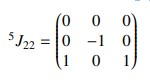
\includegraphics[scale=1]{imagenes/EC4.jpg} \\
Por tanto, la direccion singular asociada es la rotación alrededor del eje \textit{x} del sistema de referencia
{5}.\\\\\\
\textbf{Referencias:}\\
Análisis Cinemático de Robots Manipuladores Redundantes:
Aplicación a los Robots Kuka LWR 4+ y ABB Yumi
Isiah Zaplana,J. Arnau Claret, L. Basanez, 2018.\\\\
ANALISIS DE SINGULARIDAD DEL MECANISMO ESPACIAL TIPO RRRCR, J. J. Cervantes Sanchez, J. M. Rico Martínez, A. Bitangilayi, G. I. Pérez Soto, M. A. Sánchez Ruenes, 2012.
\end{document}
